%%%%%%%%%%%%%%%%%%%%%%%%%%%%%%%%%%%%%%%%%%%%%%%%%%%%%%%%%%%%%%%%%%%%%%%%%%%%%%%%%
%%%%%                           EXPERIENCED MW                               %%%%
%%%%%%%%%%%%%%%%%%%%%%%%%%%%%%%%%%%%%%%%%%%%%%%%%%%%%%%%%%%%%%%%%%%%%%%%%%%%%%%%%
Thus far we have used the statutory minimum wage as our variable of interest. More 
precisely, treatment was built as the maximum across federal, state and local minimum wage.
While the main goal is to address economic concerns related to the targeted labor market (
MW provisions provide a positive income shock to lower income workers in treated areas, conditional 
on constant employment), an important feature of MW policies is the geographical scope 
inherently associated with them.  
Since this paper focuses on the indirect impact that such policies have on 
the rental housing market at the local level, measuring the treatment intensity with the \textit{statutory} 
MW can introduce bias arising from measurement error in the main 
explanatory variable. The reason is that MW workers may not live in the same zipcode where they work. 
Taking this to an extreme, there could be zipcodes that are considered \textit{treated} (i.e. they experience a 
change in the statutory MW) while not having MW workers as residents.  At the same time, there may be 
MW workers affected by MW provisions residing in zipcodes that are not directly treated. Addressing this issue 
becomes important because, even though the majority of MW changes in the sample comes from state-level 
legislation, our identification strategy also rely on county- and city-level variation. In such context, it is more 
likely to have discrepancies between the MW variation experienced by workers at the workplace and residence 
location and, as explained in \autoref{sec:empirical_strategy}, we identify the causal effect of MW on 
rents via-variation in both the timing \textit{and} the magnitude of MW changes. 

Investigating this issue is important because, while the present version of this paper abstracts from an explicit modeling 
of the mechanism driving up prices for rental units, the reduced form evidence provided so far can be rationalized by 
assuming that a positive income shock to MW workers translates into higher demand for housing. This demand 
should then be stronger in those zipcodes where a larger share of treated workers resides. We test this assumption by 
using the 2017 LEHD Origin-Destination Employment Statistics (LODES) to create a proxy to identify, for each 
zipcode in our sample, the number of MW workers and MW residents. Specifically, we approximate such quantities
with the number of workers and residents younger than $29$ years old earning less than $\$1250$/month.\footnote{ADD 
	DETAILED DESCRIPTION OF THE PROCEDURE TO BUILD LODES-BASED MW WORKERS AND RESIDENTS SHARES}
We then compute the zipcode-level share of MW workers and residents, out of state totals. This allows us to 
geographically identify those zipcodes that constitutes either the workplace or the residence for a higher share
of MW earners. We finally estimate the differential impact on quartiles for such distributions 
using \autoref{eq:diff_main_hetero}, and we report the estimated coefficients of interest in \autoref{fig:static_qtl_lodes}.
The first thing to notice is that the effect of MW on rents does not change across zipcode with different
share of MW jobs. Coefficients shown in  \autoref{fig:static_qtl_lodes}, panel (a) all present point estimates
very close to the average static effect introduced in \autoref{tab:did_main}: a 10 percent increase in the MW leads
to a $0.26$ percent increase in rents. This therefore suggest how the causal link between MW and rent is orthogonal 
to the division of zipcodes based on the share of MW jobs they provide. The precision of such estimates however 
decreases as we go from the first to the fourth quartile, as documented by growing confidence intervals, making the 
fourth quartile's coefficient not particularly informative.\footnote{\label{ft:long_tail}This 
	is likely caused by the long right tail in the underlying distribution (\autoref{fig:lodes_share_dist}).}  
\autoref{fig:static_qtl_lodes}, panel (b) highlights, on the other hand, a positive relationship between the share of 
MW residents and the intensity of the impact of MW on rents.  Zipcodes with the lowest share of MW residents
reports a precisely estimated zero effect, while a 10 percent MW increase in the 
third quartile leads to a $0.5$ percent increase in rents. The estimated effect in the upper quartile 
diminishes to  $0.26$  and it is not statistically significant.\footnote{see footnote \ref{ft:long_tail}.}\footnote{The
use of zipcode-level state shares helps in identifying the geographical spread of MW workers/residents within 
a state. This approach however presents one drawback: there may be two zipcodes displaying the same state-level share, 
but with very different income distribution. This would imply that the richer zipcode has a lower 
\textit{relative} share of MW workers/residents out of the total zipcode population. To better identify neighborhoods with 
a higher relative concentration of MW workers/residents, we re-estimate the heterogeneous impact of MW on rents 
by using zipcode-level shares instead. Results are shown in  \autoref{fig:static_qtl_lodes2}.} 

\begin{figure}[htb!]\centering
	\caption{Effect of Minimum Wage on Rents by Quartiles of Low-income and Young Workers' share Distribution}
	\label{fig:static_qtl_lodes}
	\begin{subfigure}[b]{\textwidth}
		\caption{Workplace Distribution}
		\includegraphics[width = .7\textwidth]{../../analysis/first_differences_expmw/output/fd_static_heter_walall_29y_lowinc_ssh_st_qtl.eps}
	\end{subfigure}
	\begin{subfigure}[b]{\textwidth}
		\caption{Residential Distribution}
		\includegraphics[width = .7\textwidth]{../../analysis/first_differences_expmw/output/fd_static_heter_halall_29y_lowinc_ssh_st_qtl.eps}
	\end{subfigure}
	\begin{minipage}{\textwidth}\footnotesize
		\vspace{3mm}	
		\textit{Notes:} Panel (a) shows the estimated $\beta_q$ coefficients from \autoref{eq:diff_main_hetero},  quartiles are 
		based on the zipcode-level state share of MW workers whose workplace is found in a given zipcode. 
		Panel (b) shows the estimated $\beta_q$ coefficients from \autoref{eq:diff_main_hetero}, where quartiles are 
		based on the zipcode-level state share of MW workers whose residence is found in a given zipcode. 
		All specifications include time fixed effects, 
		and additionally use QCEW data to control for wages, employment and number of establishments 
		for the ``Professional and business services", ``Information", and ``Financial activities" industries.
		Standard errors clustered at the state level, and 90 percent confidence intervals are reported alongside 
		the estimated coefficients. 
	\end{minipage}
\end{figure}



\subsection{A new minimum wage measure}
MW policies have an increasing effect on rents for zipcodes with a higher concentration of MW residents. 
This provides an empirical justification for refining the main explanatory variable so to better account for 
the difference between the statutory MW assigned to a zipcode-month unit, and the actual MW that its 
residents are exposed to. We use the 2017 LEHD Origin-Destination Employment Statistics (LODES) to 
build a measure of \textit{experienced MW}. This summarizes the MW level faced by workers living in a certain zipcode, 
based on their workplace location. LODES data provides the number of workers for each origin-destination 
pair of U.S. Census blocks. Starting from that, we first build a zipcode-level origin-destination matrix. 
We then compute the weighted average of the MW faced by each zipcode-month cell in our final sample, 
using the number of workers commuting to each destination as weights.\footnote{We trim, for each 
	origin, the number of destination-zipcodes to those making up to 90 percent of the workforce due to 
	the high number of destinations with extremely low percentages of workers. Subsequent results 
	based on the full distribution are identical to those presented.} 

The new measure we obtain is highly correlated with the original statutory MW (98.5 percent), but it 
increases the number of treated zipcode-month observations in the sample from 5,302 to 8,942. 
As an illustration, figure \ref{fig:expmw_san_diego} plots the statutory versus experienced 
MW variables following the California increase in the minimum wage on January, 2019. As of 
December 2018 the MW in San Diego city was \$11.50, whereas the state's MW binding outside 
the city was \$11.\footnote{For employers larger than 26 employees. For those below 26 
	employees the level was \$10.50.}
The increase in the state level MW to \$12 in January 2020 appears as a discontinuity in the 
city border. However, when we account for the fact that MW workers commute, we observe a 
gradient in the intensity of the policy.

\begin{figure}
	\caption{The California MW increase of January 2019 in San Diego}
	\label{fig:expmw_san_diego}
	\centering
	\begin{subfigure}[b]{0.55\textwidth}
		\caption{Statutory MW change}
		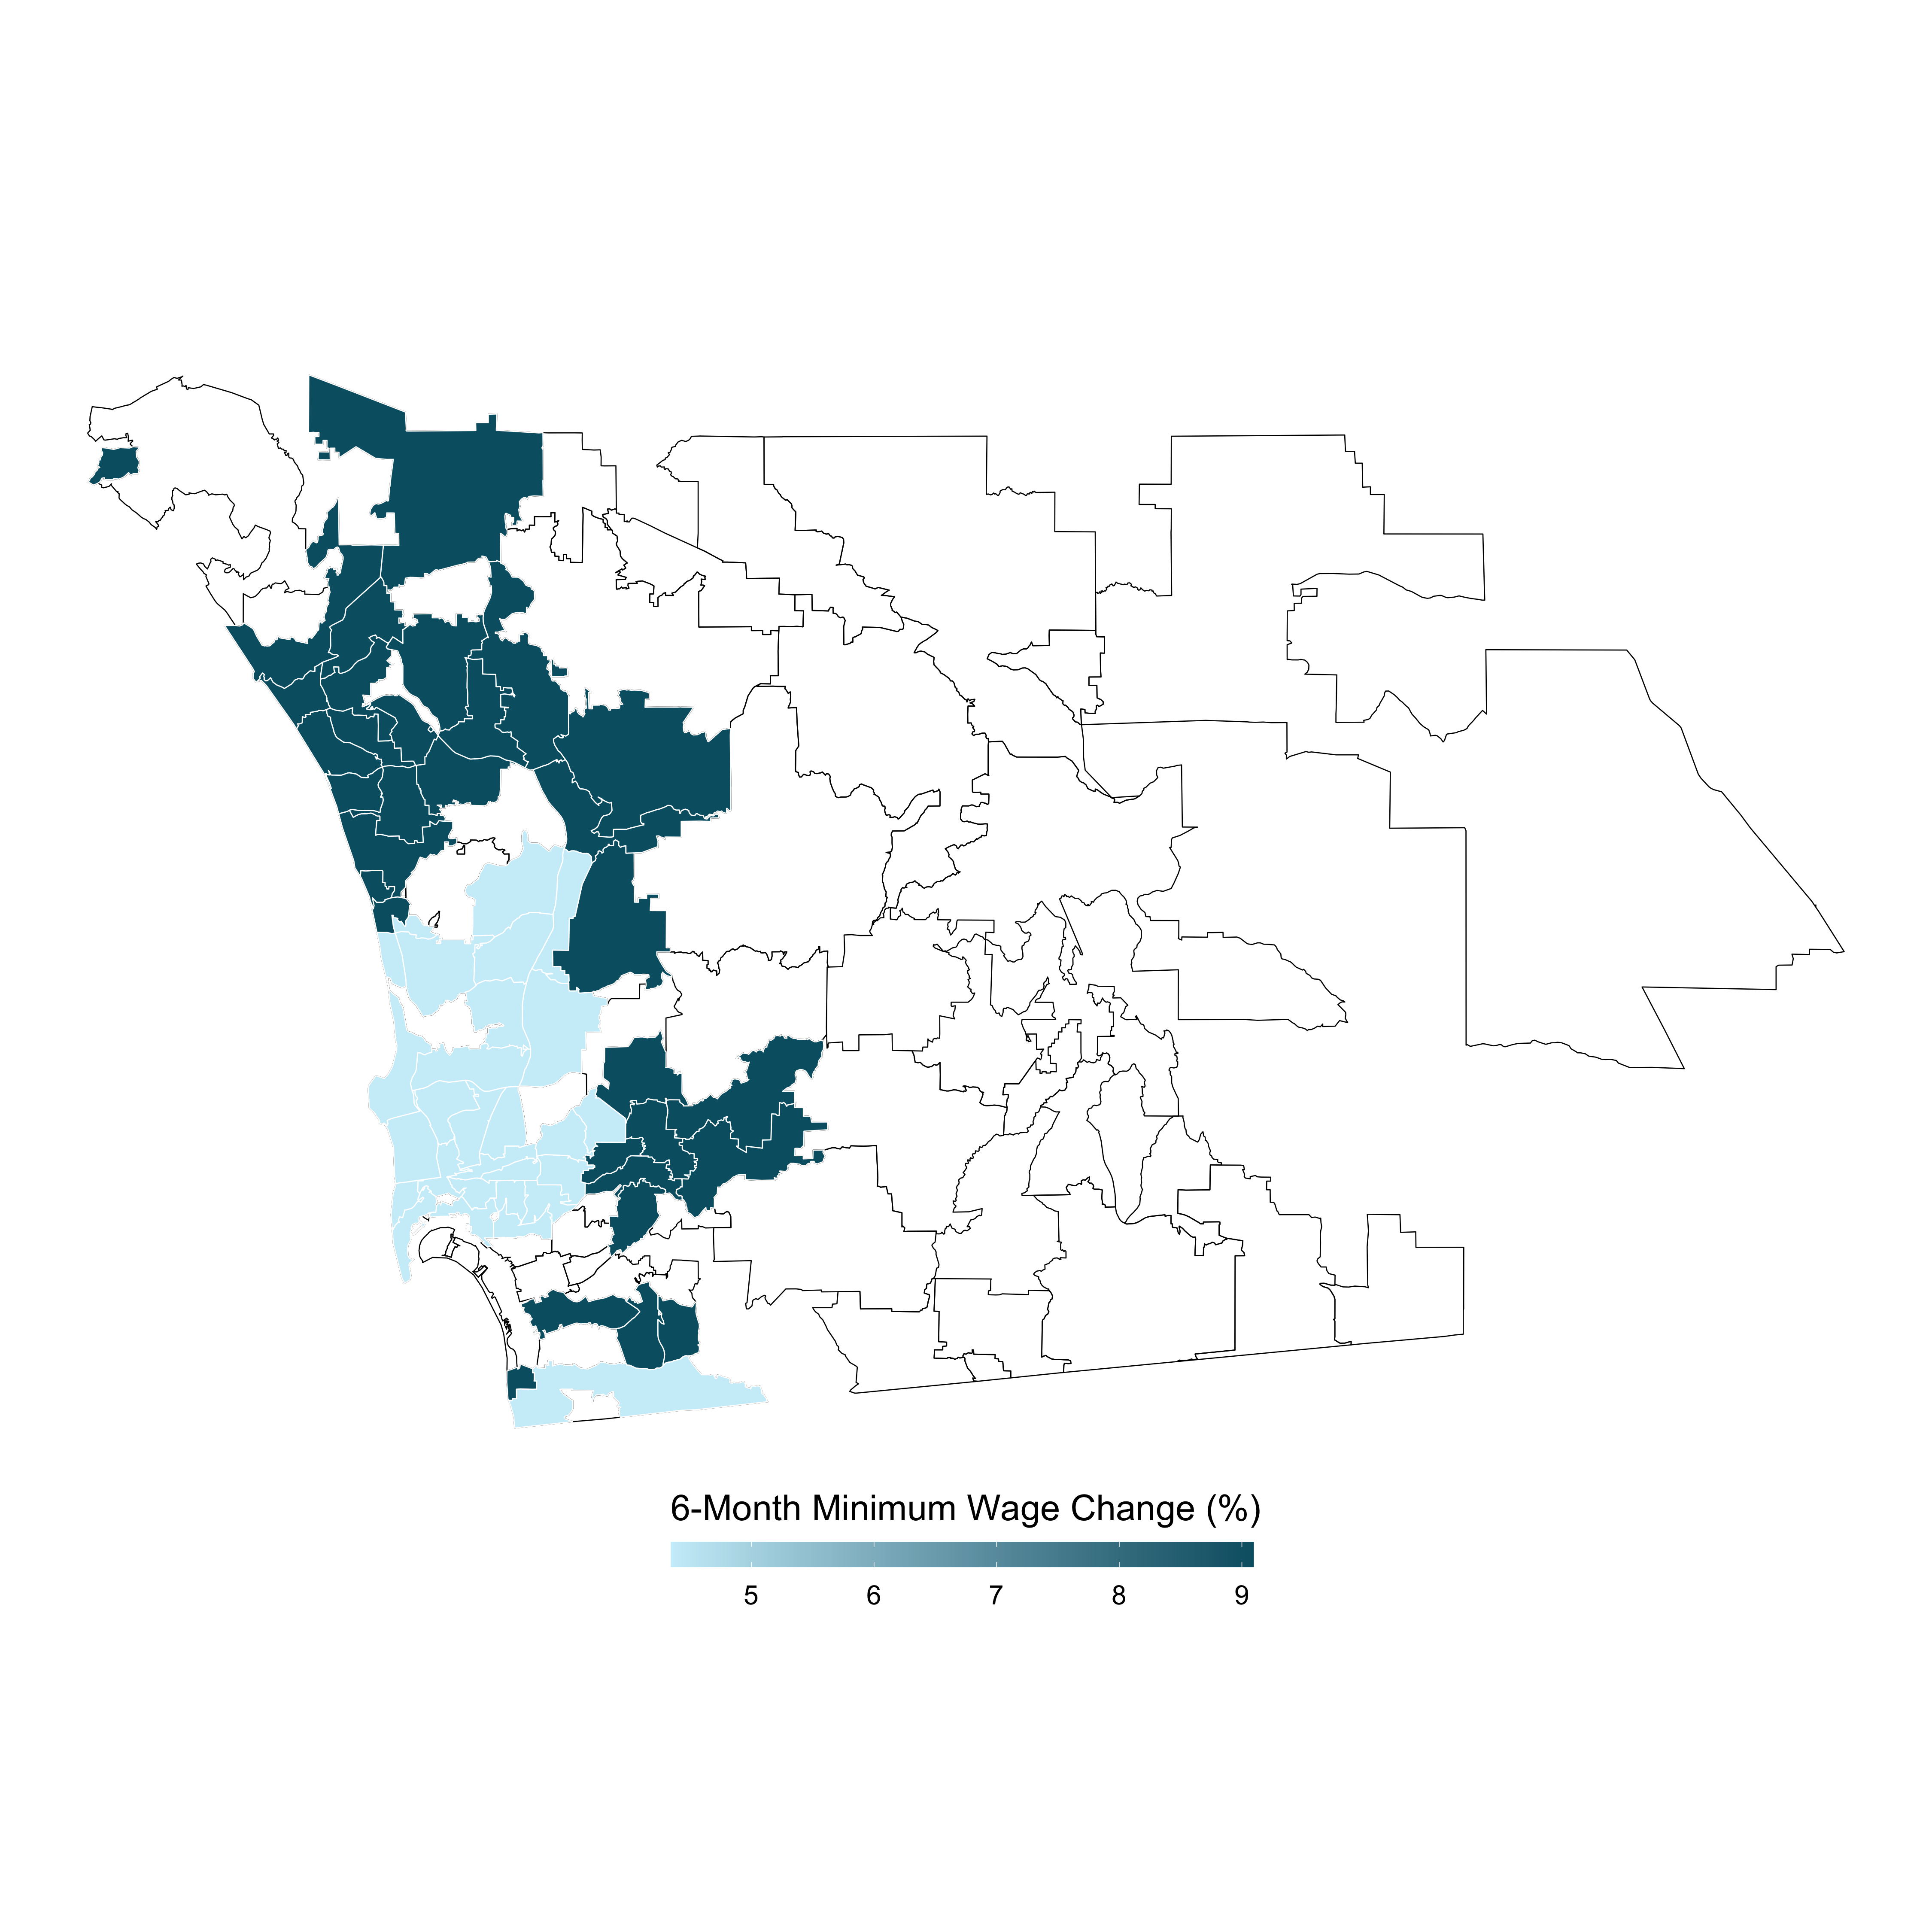
\includegraphics[width = \textwidth]
		{../../analysis/descriptive_maps/output/San_Diego_mw_msa.png}
	\end{subfigure}
	\begin{subfigure}[b]{0.55\textwidth}
		\caption{Experienced MW change}
		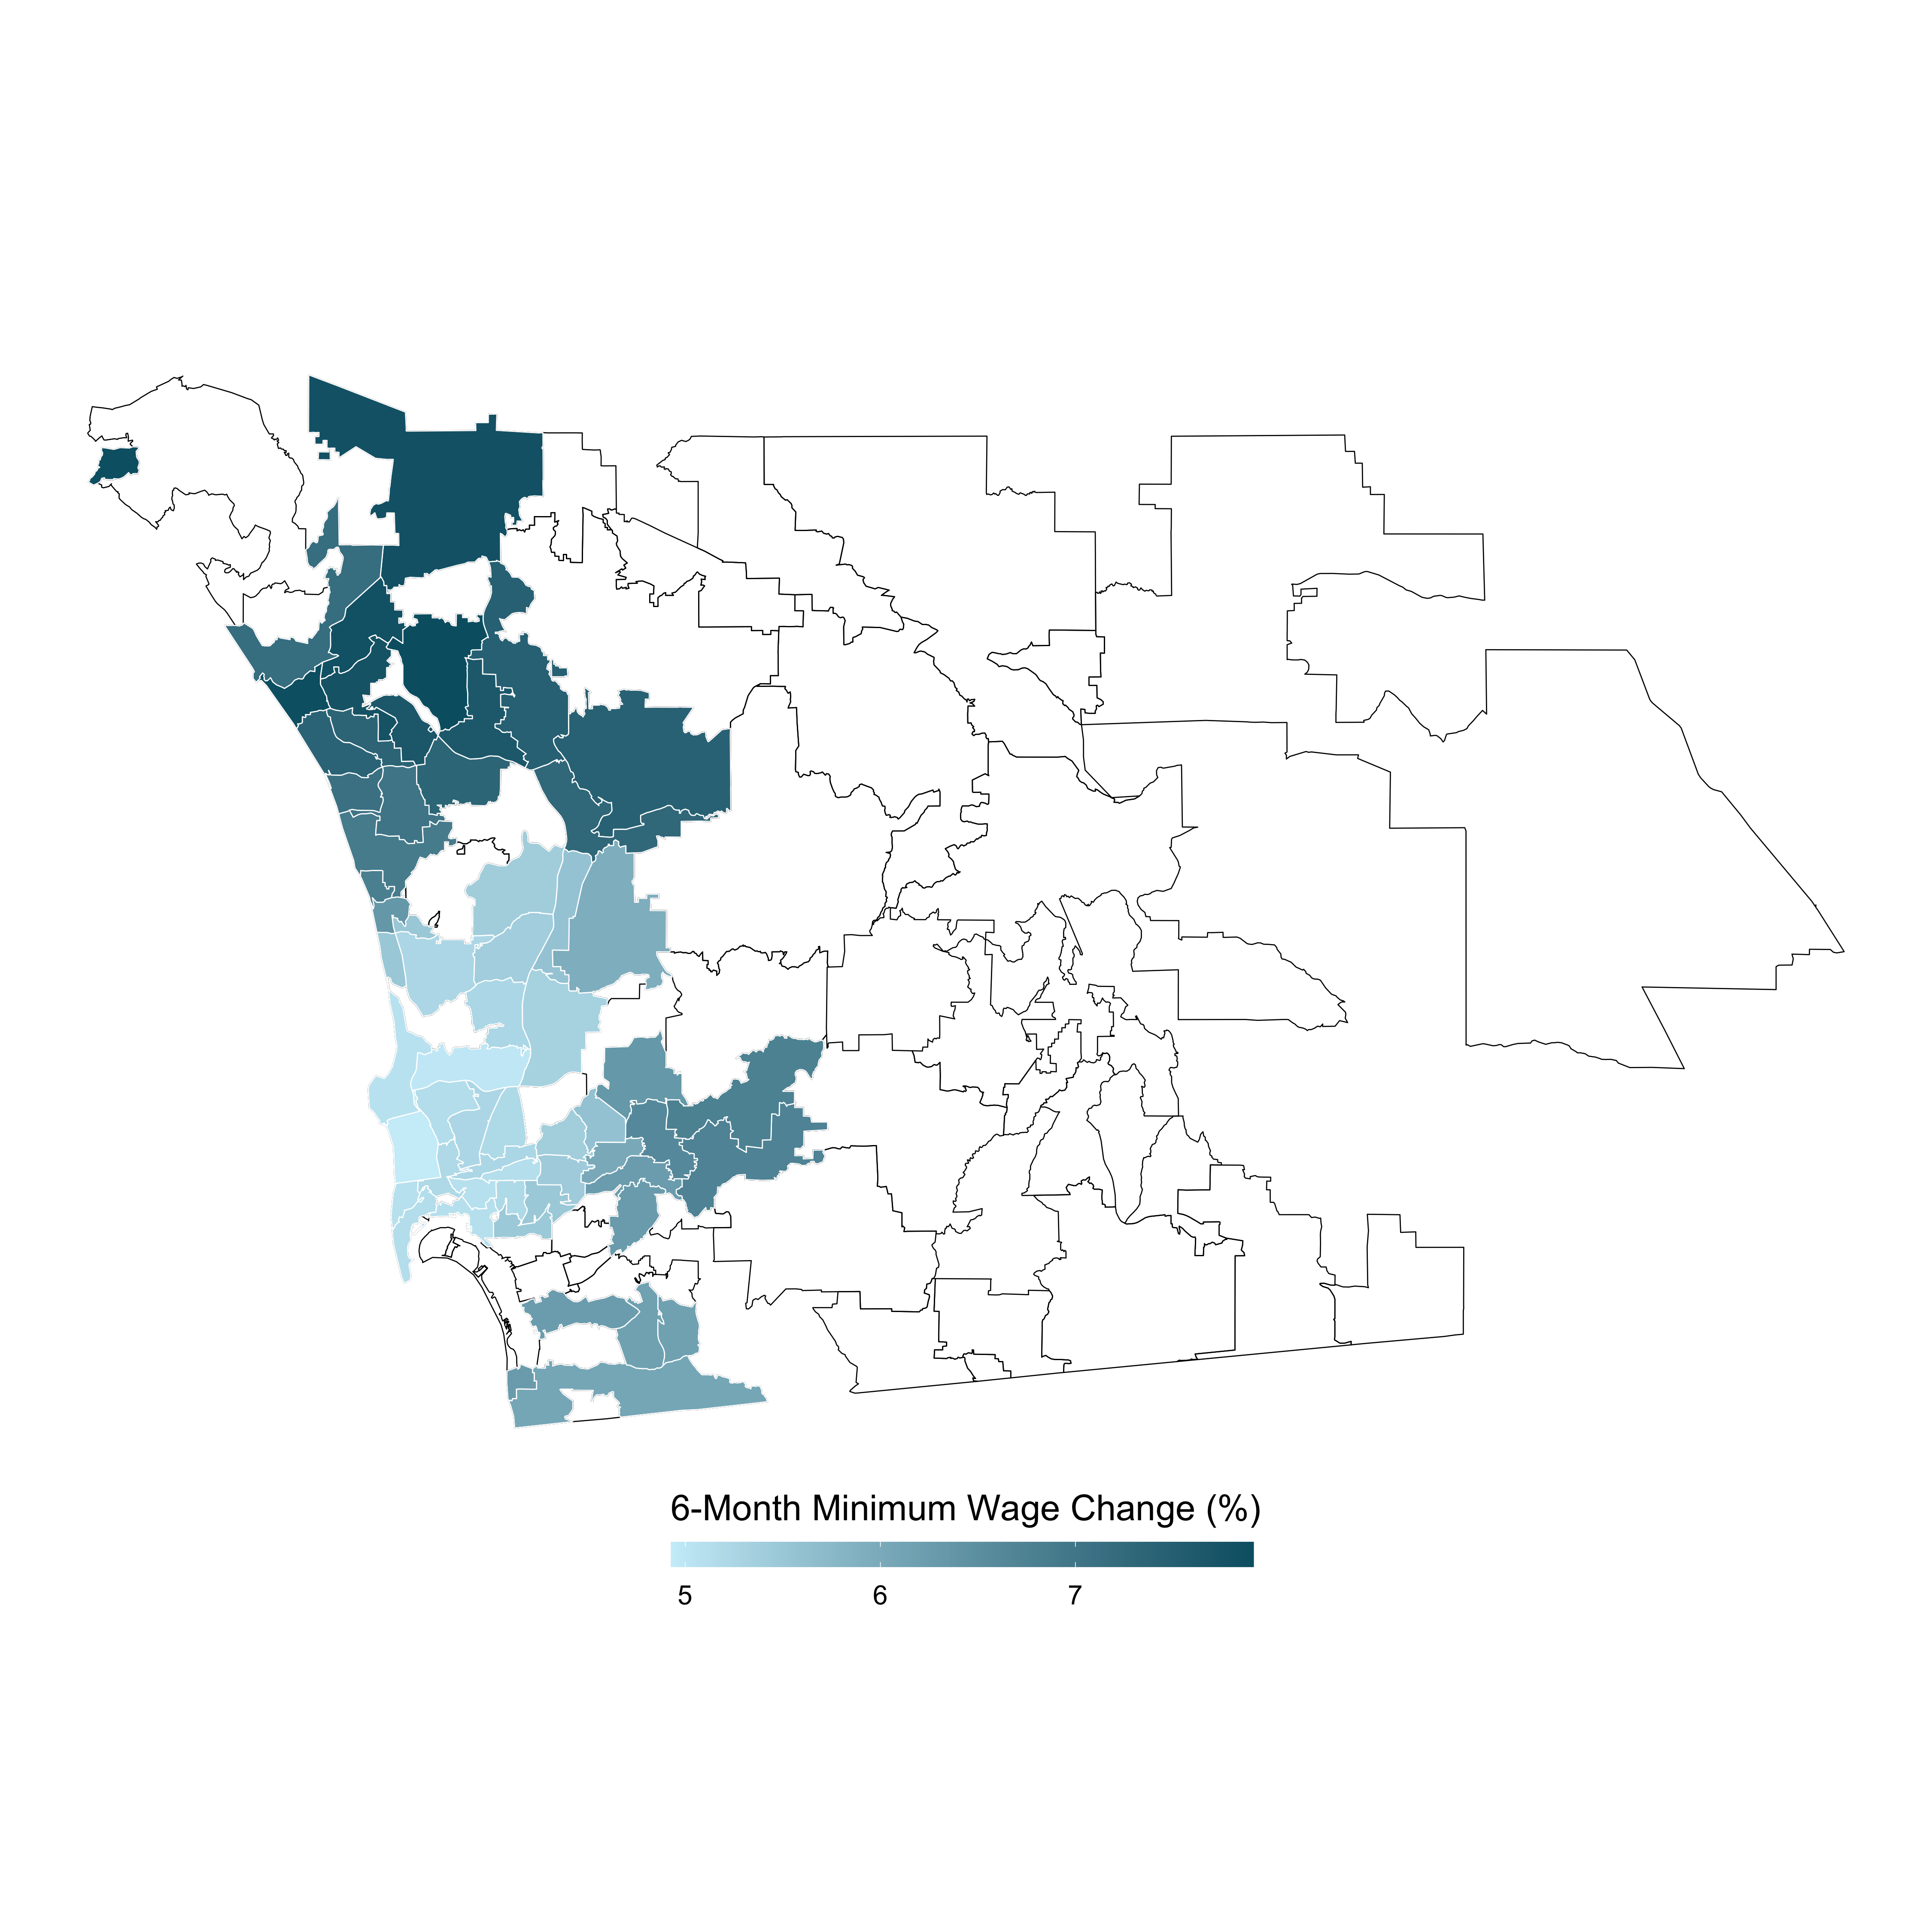
\includegraphics[width = \textwidth]
		{../../analysis/descriptive_maps/output/San_Diego_expmw_msa.png}
	\end{subfigure}
	\begin{minipage}{0.95\textwidth} \footnotesize
		\vspace{2mm} 
		\textit{Notes}: The figure maps the percent increase in our minimum wage and 
		experienced minimum wage measures following the state increase in California
		on January 2019. The map colors only zipcodes for which we have non-missing 
		rents data from Zillow.
	\end{minipage}
\end{figure}


%%%%%%%%%%%%%%%%%%%%%%%%%%%%%%%%%%%%%%%%%%%%%%%%%%%%%%%%%%%%%%%%%%%%%%%%%%%%%%%%%
\subsection{Estimation results}

We then re-estimate our baseline model using the experienced MW as treatment variable and present the results in \autoref{fig:expmw_dynamic}. The estimated effect of MW on rents slightly increases in the two statistically significant periods,  $t=0$ and $t=1$, but the new results largely confirm the magnitude and dynamics uncovered by the baseline model. A 10 percent increase in experienced MW leads to a $0.31$ percent contemporaneous increase in median rents, as well as a $0.145$ increase in the following month. The absence of statistically significant pre-trend is confirmed.    

\begin{figure}[!h]
	\centering
	\caption{Estimated Impact of changes in Experienced MW on changes in Rents - Dynamic DiD model}
	\label{fig:expmw_dynamic}
	\includegraphics[width = .9\textwidth]{../../analysis/first_differences_expmw/output/fd_model_comparison_expmw.eps}
	\begin{minipage}{.9\textwidth}\footnotesize
		\textit{Notes:} The figure compares the estimated $\beta_{k}$ coefficients from \autoref{eq:leads_lags} for the baseline model and those obtained while replacing the statutory MW with the experienced MW. The solid lines report the point estimates for the cumulative effect implied by a model with lags only.  
	\end{minipage}
\end{figure}


